
% !TEX program = pdflatex
\documentclass[aspectratio=169,10pt]{beamer}

% ----------------------
% Theme / look
% ----------------------
\usetheme{Madrid}
\usecolortheme{default}
\setbeamertemplate{navigation symbols}{}
\setbeamertemplate{caption}[numbered]
\usefonttheme{professionalfonts}

% ----------------------
% Packages
% ----------------------
\usepackage{amsmath,amssymb,bm,mathtools}
\usepackage{graphicx}
\usepackage{booktabs,tabularx,array}
\usepackage{siunitx}
\usepackage{tikz}
\usepackage{pgfplots}
\pgfplotsset{compat=1.18}
\usetikzlibrary{arrows.meta,positioning,calc,patterns}

\usepackage[most]{tcolorbox}
\usepackage{listings}
\usepackage{xcolor}

% ----------------------
% Graphics
% ----------------------
\graphicspath{{Figures/}}

% ----------------------
% Listings (MATLAB)
% ----------------------
\lstdefinelanguage{Matlab}{
  keywords={break,case,catch,continue,else,elseif,end,for,function,global,if,otherwise,persistent,return,switch,try,while},
  morekeywords={ctrb,obsv,rank,size,disp,clear,clc,eye,diag,eig,fprintf},
  sensitive=true,
  morecomment=[l]\%,
  morestring=[m]'
}
\lstset{
  language=Matlab,
  basicstyle=\ttfamily\scriptsize,
  keywordstyle=\color{blue!70!black}\bfseries,
  commentstyle=\color{green!40!black},
  stringstyle=\color{orange!70!black},
  numbers=left,
  numberstyle=\tiny\color{gray!70},
  numbersep=6pt,
  showstringspaces=false,
  breaklines=true,
  frame=single,
  rulecolor=\color{gray!40}
}

% ----------------------
% Box styles
% ----------------------
\tcbset{
  beamer,
  enhanced,
  colback=white,
  colframe=blue!60!black,
  boxrule=0.6pt,
  arc=2pt,
  left=5pt,right=5pt,top=4pt,bottom=4pt
}
\newtcolorbox{defnbox}[1]{title=#1, colframe=blue!70!black, colback=blue!3}
\newtcolorbox{notebox}[1]{title=#1, colframe=teal!70!black, colback=teal!3}
\newtcolorbox{examplebox}[1]{title=#1, colframe=orange!80!black, colback=orange!3}
\newtcolorbox{alertbox}[1]{title=#1, colframe=red!75!black, colback=red!4}
\newtcolorbox{summarybox}[1]{title=#1, colframe=purple!70!black, colback=purple!4}

% ----------------------
% Convenience macros
% ----------------------
\newcommand{\R}{\mathbb{R}}
\newcommand{\T}{^\top}
\newcommand{\Ccal}{\mathcal{C}}
\newcommand{\Ocal}{\mathcal{O}}

% ----------------------
% Metadata
% ----------------------
\title[Controllability \& Observability]{Controllability \& Observability}
\subtitle{MSc Model Predictive Control}
\author{(Your name)}
\institute{(Your institution)}
\date{\today}

\begin{document}

% =========================================================
% Title
% =========================================================
\begin{frame}
\titlepage
\end{frame}

\begin{frame}{A guiding thought}
\begin{quote}
\itshape
``To control a physical system, we must first determine whether the available inputs can influence the state,
and whether the available outputs contain sufficient information to reconstruct it.''
\end{quote}
\end{frame}

% =========================================================
% Motivation
% =========================================================
\section{Motivation}

\begin{frame}{Why do we need controllability and observability?}
In previous chapters, we focused on \textbf{optimisation}: choosing the best input sequence to minimise a cost.
Before asking \emph{``what is optimal?''} we must ask something more fundamental:

\begin{center}
\textbf{Does a feasible trajectory even exist?}
\end{center}

Two structural properties answer this:
\begin{itemize}
  \item \textbf{Controllability} (actuation): can inputs steer the state where we want?
  \item \textbf{Observability} (sensing): can outputs reveal the internal state?
\end{itemize}

\begin{alertbox}{Key message}
If a system is uncontrollable or unobservable, no sophisticated MPC/LQR algorithm can overcome that limitation.
\end{alertbox}
\end{frame}

\begin{frame}{Controllability vs observability: the twin questions}
\begin{columns}[T,totalwidth=\textwidth]
\begin{column}{0.5\textwidth}
\begin{defnbox}{Controllability (actuation)}
Given \(x_{k+1}=Ax_k+Bu_k\), can we steer from any \(x_0\) to any target \(x_N\) using a finite input sequence?
\end{defnbox}
\vspace{0.3em}
\begin{itemize}
  \item depends on the pair \((A,B)\)
  \item about \emph{reachability} of states
  \item prerequisite for controller design (pole placement, LQR)
\end{itemize}
\end{column}
\begin{column}{0.5\textwidth}
\begin{defnbox}{Observability (sensing)}
Given \(y_k=Cx_k+Du_k\), can we uniquely reconstruct \(x_0\) from knowledge of \(u\) and \(y\) over a finite horizon?
\end{defnbox}
\vspace{0.3em}
\begin{itemize}
  \item depends on the pair \((A,C)\)
  \item about \emph{information flow} to sensors
  \item prerequisite for observers (e.g. Kalman filters)
\end{itemize}
\end{column}
\end{columns}
\end{frame}

% =========================================================
% Controllability
% =========================================================
\section{Controllability}

\begin{frame}{Controllability: the core question}
Given the discrete-time LTI model
\[
x_{k+1}=Ax_k+Bu_k,
\]
the fundamental question is:

\begin{center}
\emph{Do the actuators (matrix \(B\)) have sufficient authority to influence all state directions governed by \(A\)?}
\end{center}

Trivial case:
\begin{itemize}
  \item If \(B=0\), then \(u_k\) has no effect \(\Rightarrow\) uncontrollable.
\end{itemize}

Non-trivial case:
\begin{itemize}
  \item Even with \(B\neq 0\), actuation can be restricted to a subspace.
\end{itemize}
\end{frame}

\begin{frame}{Definition of controllability}
\begin{defnbox}{Definition: Controllability}
A system is \emph{controllable} if, for any initial state \(x_0\) and any target state \(x_N\),
there exists a finite input sequence \(\{u_0,u_1,\dots,u_{N-1}\}\) that drives the system from \(x_0\) to \(x_N\).
\end{defnbox}

\begin{notebox}{Interpretation}
Controllability is an \textbf{existence} condition (not an optimisation criterion).
\end{notebox}
\end{frame}

\subsection{Derivation of the rank condition}

\begin{frame}{Expanding the dynamics (recursive substitution)}
Starting from \(x_{k+1}=Ax_k+Bu_k\), expand:
\begin{align*}
x_1 &= Ax_0+Bu_0,\\
x_2 &= Ax_1+Bu_1 = A(Ax_0+Bu_0)+Bu_1 = A^2x_0 + ABu_0 + Bu_1,\\
&\vdots\\
x_N &= A^N x_0 + \sum_{i=0}^{N-1} A^{N-1-i}B u_i.
\end{align*}

Goal: can we choose inputs to make \(x_N\) equal to any desired target?
\end{frame}

\begin{frame}{Stacking inputs and defining \(\mathcal{C}_N\)}
Rearrange:
\[
x_N - A^N x_0 = \sum_{i=0}^{N-1} A^{N-1-i}B u_i.
\]

Stack inputs into
\[
\mathcal{U}=
\begin{bmatrix}
u_{N-1}\\u_{N-2}\\\vdots\\u_0
\end{bmatrix},
\]
and define
\[
x_N - A^N x_0 =
\underbrace{\begin{bmatrix}
B & AB & A^2B & \cdots & A^{N-1}B
\end{bmatrix}}_{\mathcal{C}_N}
\mathcal{U}.
\]

This is a linear system \(b=\mathcal{C}_N\mathcal{U}\) where \(b=x_N-A^N x_0\).
\end{frame}

\begin{frame}{Controllability as a solvability problem}
\begin{alertbox}{Key question}
Does a solution \(\mathcal{U}\) exist for \emph{any} desired vector \(b\in\R^n\)?
\end{alertbox}

This holds iff the columns of \(\mathcal{C}_N\) span \(\R^n\), i.e.
\[
\mathrm{rank}(\mathcal{C}_N)=n.
\]

But \(\mathcal{C}_N\) grows with \(N\). We need a finite test.
\end{frame}

\begin{frame}{Why we only need \(n\) blocks (Cayley--Hamilton)}
Let \(n=\dim(x)\).
By the \textbf{Cayley--Hamilton theorem}, higher powers of \(A\) do not add new independent directions:
\[
A^k\ (k\ge n)\ \text{is a linear combination of}\ I,A,\dots,A^{n-1}.
\]

Therefore, define the standard controllability matrix
\[
\Ccal=\begin{bmatrix}
B & AB & A^2B & \cdots & A^{n-1}B
\end{bmatrix}.
\]
\end{frame}

\begin{frame}{Kalman rank condition (controllability)}
\begin{alertbox}{Theorem: Kalman rank condition}
The pair \((A,B)\) is controllable iff
\[
\mathrm{rank}(\Ccal)=n,
\quad
\Ccal=\begin{bmatrix}B & AB & \cdots & A^{n-1}B\end{bmatrix}.
\]
\end{alertbox}

\textbf{Interpretation:}
\begin{itemize}
  \item columns of \(\Ccal\) span \(\R^n\),
  \item there is no state subspace immune to actuation.
\end{itemize}
\end{frame}

\subsection{Controllability in MATLAB}

\begin{frame}{Controllability in MATLAB: discrete-time double integrator}
Discrete-time double integrator (sampling time \(h\)):
\[
A=\begin{bmatrix}1 & h\\0 & 1\end{bmatrix},
\qquad
B=\begin{bmatrix}\tfrac{1}{2}h^2\\h\end{bmatrix}.
\]

Best practice: use \texttt{ctrb(A,B)} to form \(\Ccal\), and check \(\mathrm{rank}(\Ccal)\).
\end{frame}

\begin{frame}[fragile]{MATLAB: controllability check with \texttt{ctrb}}
\begin{lstlisting}[caption={Checking controllability using \texttt{ctrb}.}]
% Discrete-time double integrator
h = 0.1;
A = [1, h;
     0, 1];

B = [0.5*h^2;
     h];

n = size(A, 1);

Co = ctrb(A, B);
rank_Co = rank(Co);

fprintf('State Dimension n = %d\n', n);
fprintf('Rank of Co      = %d\n', rank_Co);
\end{lstlisting}
\end{frame}

\begin{frame}{Interpreting the controllability result}
If \(\mathrm{rank}(\Ccal)=n\), then:
\begin{itemize}
  \item an input sequence exists to move between any states (ignoring constraints),
  \item state-feedback design is structurally feasible.
\end{itemize}

For the double integrator, typically \(n=2\) and \(\mathrm{rank}(\Ccal)=2\) \(\Rightarrow\) controllable.

\begin{notebox}{Important caveat}
Controllability is structural. Constraints (saturation, rate limits) can still prevent reaching some targets.
\end{notebox}
\end{frame}

% =========================================================
% Observability
% =========================================================
\section{Observability}

\begin{frame}{Observability: reconstructing the state from outputs}
Observability is the inverse problem:
\begin{itemize}
  \item controllability: choose \(u\) to affect \(x\),
  \item observability: use \(u\) and \(y\) to infer \(x\).
\end{itemize}

Most advanced controllers require full state feedback (or a state estimate):
\[
u_k = -K\hat{x}_k
\quad \text{or} \quad
u_k = \pi(\hat{x}_k).
\]

If not all states are measured, we design an \textbf{observer}.
Observability tells us whether this is possible.
\end{frame}

\begin{frame}{Definition of observability}
\begin{defnbox}{Definition: Observability}
A linear system is \textbf{observable} if the initial state \(x(t_0)\) can be uniquely determined
from knowledge of the input \(u(t)\) and output \(y(t)\) over a finite time interval.
\end{defnbox}

If a system is unobservable, there exists at least one internal mode that does not influence the output.
\end{frame}

\subsection{Observability matrix}

\begin{frame}{The observability matrix}
For an LTI system, define
\[
\Ocal=
\begin{bmatrix}
C\\
CA\\
CA^2\\
\vdots\\
CA^{n-1}
\end{bmatrix}.
\]

\begin{notebox}{Kalman rank condition (observability)}
The pair \((A,C)\) is observable iff
\[
\mathrm{rank}(\Ocal)=n.
\]
\end{notebox}

If the rank is less than \(n\), there are state directions that cannot be determined from measurements.
\end{frame}

\begin{frame}{Example: an unobservable system (rank deficiency)}
System:
\begin{align*}
\dot{x} &= \begin{bmatrix}-1 & 0\\0 & -2\end{bmatrix}x + \begin{bmatrix}1\\1\end{bmatrix}u,\\
y &= \begin{bmatrix}1 & 0\end{bmatrix}x.
\end{align*}

Compute
\[
\Ocal=
\begin{bmatrix}
C\\CA
\end{bmatrix}
=
\begin{bmatrix}
1 & 0\\
-1 & 0
\end{bmatrix}.
\]

Second column is zero \(\Rightarrow\) \(x_2\) never affects \(y\).
Thus \(\mathrm{rank}(\Ocal)=1<2\) \(\Rightarrow\) not observable.
\end{frame}

\begin{frame}{Why unobservability is dangerous}
If an unobservable mode is unstable:
\begin{itemize}
  \item internal state can diverge,
  \item output may not show it,
  \item controller/estimator cannot correct what it cannot see.
\end{itemize}

\begin{alertbox}{Engineering warning}
Unobservable unstable modes can lead to catastrophic failures that are not detectable from the available sensors.
\end{alertbox}
\end{frame}

\subsection{Derivation via stacking measurements (DT)}

\begin{frame}{Deriving the observability test by stacking outputs}
For intuition, subtract the forced response (inputs are known) and consider
\[
x_{k+1}=Ax_k,\qquad y_k=Cx_k.
\]

Then:
\begin{align*}
y_0 &= Cx_0,\\
y_1 &= CAx_0,\\
y_2 &= CA^2x_0,\\
&\vdots\\
y_{n-1} &= CA^{n-1}x_0.
\end{align*}

Stacking:
\[
Y=
\begin{bmatrix}
y_0\\y_1\\\vdots\\y_{n-1}
\end{bmatrix}
=
\underbrace{
\begin{bmatrix}
C\\CA\\\vdots\\CA^{n-1}
\end{bmatrix}}_{\Ocal}
x_0
= \Ocal x_0.
\]
\end{frame}

\begin{frame}{Invertibility and the rank condition}
To uniquely solve for \(x_0\) from \(Y=\Ocal x_0\), the columns of \(\Ocal\) must be independent:
\[
\mathrm{rank}(\Ocal)=n.
\]

\begin{summarybox}{Rank test and reconstruction}
If \(\mathrm{rank}(\Ocal)=n\), then one (least-squares) reconstruction is
\[
x_0 = (\Ocal^\top \Ocal)^{-1}\Ocal^\top Y.
\]
\end{summarybox}

As with controllability, Cayley--Hamilton implies we do not gain new independent information beyond \(A^{n-1}\).
\end{frame}

\subsection{Observability in MATLAB}

\begin{frame}{Observability in MATLAB: double integrator with two sensors}
We test observability for the discrete-time double integrator with two measurement choices:
\begin{enumerate}
\item Position sensor: \(C_1=[1\ \ 0]\) (measure position).
\item Velocity sensor: \(C_2=[0\ \ 1]\) (measure velocity).
\end{enumerate}

Intuition:
\begin{itemize}
  \item Measuring position over time reveals velocity (by differences).
  \item Measuring velocity alone does \emph{not} reveal absolute position (unknown offset).
\end{itemize}
\end{frame}

\begin{frame}[fragile]{MATLAB: observability check with \texttt{obsv}}
\begin{lstlisting}[caption={Comparing observability for two sensor configurations.}]
h = 0.1;
A = [1, h;
     0, 1];
n = size(A, 1);

% Case 1: position sensor
C1 = [1, 0];
Ob1 = obsv(A, C1);
rank_Ob1 = rank(Ob1);

% Case 2: velocity sensor
C2 = [0, 1];
Ob2 = obsv(A, C2);
rank_Ob2 = rank(Ob2);

disp(rank_Ob1);
disp(rank_Ob2);
\end{lstlisting}
\end{frame}

\begin{frame}{Interpreting the observability results}
Typically:
\begin{itemize}
  \item \(C_1=[1\ 0]\): \(\mathrm{rank}(\Ocal)=2\) \(\Rightarrow\) observable.
  \item \(C_2=[0\ 1]\): \(\mathrm{rank}(\Ocal)=1\) \(\Rightarrow\) not observable.
\end{itemize}

\textbf{Meaning:}
\begin{itemize}
  \item With position measurements, both position and velocity can be inferred.
  \item With only velocity measurements, absolute position cannot be recovered without extra information.
\end{itemize}

\begin{notebox}{Practical takeaway}
Always check observability before designing a state estimator.
\end{notebox}
\end{frame}

% =========================================================
% Wrap-up
% =========================================================

\section{Geometric intuition and pitfalls}

\begin{frame}{Geometric intuition: reachable and hidden subspaces}
\begin{columns}[T,totalwidth=\textwidth]
\begin{column}{0.5\textwidth}
\begin{defnbox}{Controllability: reachable subspace}
The columns of
\[
\Ccal=[B\ AB\ A^2B\ \cdots\ A^{n-1}B]
\]
span the set of state directions that can be generated by the input sequence.

If this span is all of \(\R^n\), then every state direction is reachable.
\end{defnbox}

\begin{center}
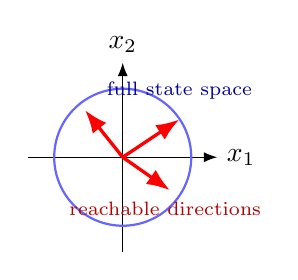
\begin{tikzpicture}[scale=0.6, >=Latex]
  \draw[->] (-2,0) -- (2,0) node[right] {$x_1$};
  \draw[->] (0,-2) -- (0,2) node[above] {$x_2$};

  % full state space
  \draw[thick, blue!60] (0,0) circle (1.45);
  \node[blue!60!black] at (1.2,1.4) {\scriptsize full state space};

  % reachable directions
  \draw[very thick, red, ->] (0,0) -- (1.2,0.8);
  \draw[very thick, red, ->] (0,0) -- (-0.8,1.0);
  \draw[very thick, red, ->] (0,0) -- (1.0,-0.7);

  \node[red!70!black] at (0.9,-1.1) {\scriptsize reachable directions};
\end{tikzpicture}
\end{center}
\end{column}

\begin{column}{0.5\textwidth}
\begin{defnbox}{Observability: hidden subspace}
If \(\mathrm{rank}(\Ocal)<n\), then there exists a nonzero vector \(v\) such that
\[
\Ocal v = 0.
\]
That means motion along \(v\) leaves no trace in the output history.
\end{defnbox}

\begin{center}
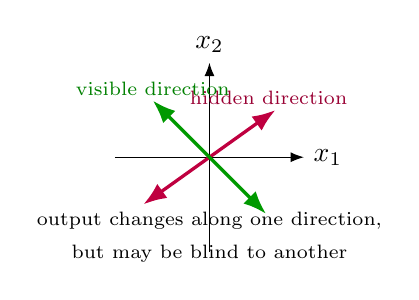
\begin{tikzpicture}[scale=0.6, >=Latex]
  \draw[->] (-2,0) -- (2,0) node[right] {$x_1$};
  \draw[->] (0,-2) -- (0,2) node[above] {$x_2$};

  % hidden direction
  \draw[very thick, purple, <->] (-1.4,-1.0) -- (1.4,1.0);
  \node[purple!80!black] at (1.25,1.25) {\scriptsize hidden direction};

  % measured direction
  \draw[very thick, green!60!black, <->] (-1.2,1.2) -- (1.2,-1.2);
  \node[green!50!black] at (-1.2,1.45) {\scriptsize visible direction};

  \node[align=center] at (0,-1.7) {\scriptsize output changes along one direction,\\ \scriptsize but may be blind to another};
\end{tikzpicture}
\end{center}
\end{column}
\end{columns}
\end{frame}

\begin{frame}{Common pitfalls and misconceptions}
\begin{itemize}
  \item \textbf{Controllable does not mean easy to control.}\\
  A controllable system may still require huge inputs, long horizons, or violate actuator constraints.

  \item \textbf{Observable does not mean easy to estimate numerically.}\\
  A system may be theoretically observable but very poorly conditioned in practice.

  \item \textbf{Rank tests are structural, not performance tests.}\\
  They answer ``possible or impossible?'', not ``fast, robust, or well-conditioned?''

  \item \textbf{Unconstrained controllability is weaker than constrained feasibility.}\\
  MPC may still become infeasible because of state/input bounds.

  \item \textbf{Sensor choice matters enormously.}\\
  Measuring the ``wrong'' variable can make an otherwise simple system unobservable.

  \item \textbf{Discrete-time and continuous-time tests are analogous but not identical.}\\
  Always check the correct pair \((A,B)\) or \((A,C)\) for the model you are actually using.
\end{itemize}

\begin{alertbox}{Practical lesson}
Before designing an MPC controller or estimator, always check controllability/observability first, then examine conditioning, constraints, and noise sensitivity.
\end{alertbox}
\end{frame}


\section{Key takeaways}

\begin{frame}{Key takeaways}
\begin{itemize}
  \item Controllability and observability are \textbf{existence conditions} for control/estimation.
  \item Controllability matrix:
  \[
  \Ccal=[B\ AB\ \dots\ A^{n-1}B],\quad \mathrm{rank}(\Ccal)=n.
  \]
  \item Observability matrix:
  \[
  \Ocal=\begin{bmatrix}C\\CA\\\vdots\\CA^{n-1}\end{bmatrix},\quad \mathrm{rank}(\Ocal)=n.
  \]
  \item If uncontrollable: some state directions cannot be influenced by input.
  \item If unobservable: some internal modes cannot be inferred from output history.
  \item MPC/LQR require (at least) controllability for regulation and observability for state estimation.
\end{itemize}
\end{frame}

\begin{frame}{Bridge to observers and output-feedback control}
Typical next steps:
\begin{itemize}
  \item If \((A,C)\) is observable: design an observer/Kalman filter to compute \(\hat{x}_k\).
  \item If \((A,B)\) is controllable: design a feedback law (LQR) or an MPC controller.
  \item Combine estimation + control \(\Rightarrow\) output-feedback implementation.
\end{itemize}

\begin{center}
\textbf{You cannot optimise what you cannot reach or observe.}
\end{center}
\end{frame}

\end{document}
